% momentum
\section{Kraftar sem vigrar}
Kraftar í einni vídd eru hagnýtir, nema það er oft þörf að taka mark á fleiri
en einni vídd, vídd hér er átt við hreyfistefna. Kraftur sem verkar á horni er
hægt að lýsa sem tveim kröftum sem eru hornréttir á hvorn annan. Almennt getum 
við sagt að kraftur er gefinn í hornréttu hnitakerfi er
\begin{align}
	\uforce_\text{x} &= \uforce \cos(\theta)\\
	\uforce_\text{y} &= \uforce \sin(\theta)
\end{align}
Þar sem $\uforce$ táknar stærð vigursins, $\uforce_\text{x}$ táknar stærð vigurs 
meðfram x-ás og $\uforce_\text{y}$ táknar stærð vigurs meðfram y-ás. Almennt er
hægt að gera þetta við alla vigra, ekki einungis kraftvigra, þeir vigrar sem munu
verða skoðaðir í þessum hluta eru kraftvigrar. Mynd \ref{basic:fig:twodimforces}
sýnir dæmi um hvernig kraftur er þáttum meðal ásum kerfisins.

Ef kassi er togaður áfram og togáttin er samsíða planinu sem kassi er dreginn eftir
þá fer allur togkraftur í að toga kassann áfram. Hins vegar ef kassi er dreginn
á horni við planið, þá er hluti af togkraftinum sem fer í að toga kassann áfram
og hluti fer í að lyfta kassann upp.

\begin{figure}[!htb]
\label{basic:fig:twodimforces}
\centering
\def\iangle{35} % Angle of the inclined plane
\def\down{-90}
\def\arcr{0.45cm} % Radius of the arc used to indicate angles
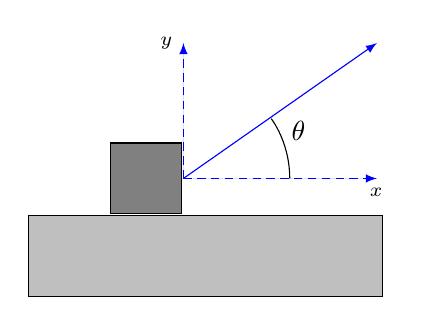
\begin{tikzpicture}[
	force/.style={>=latex,draw=blue,fill=blue},
	forcecomp/.style={>=latex,draw=blue, densely dashed, fill=blue},
	axis/.style={densely dashed,gray,font=\small},
	m/.style={rectangle,draw=black,fill=gray,minimum size=0.3cm,thin},
	scale= 3
]
	\node[m, transform shape] (m) {};
	\draw[force,->] (m.east) -- +({cos(\iangle)},{sin(\iangle)}) node[right] {$\uforce_\text{}$};
	% Indicate angle. The code is a bit awkward.
	\draw[forcecomp,->] (m.east) -- +({cos(\iangle)},0) node[below] {$\uforce_\text{x}$};
	\draw[forcecomp,->] (m.east) -- +(0,{sin(\iangle)}) node[left] {$\uforce_\text{y}$};
	\draw[solid,shorten >=0.5pt] (m.east) +(0:\arcr)
		arc(0:\iangle:\arcr);
	\node at (0+\iangle*0.5:1.5*\arcr) {$\theta$};
	\node[] (table) {};
	\draw[draw=black, fill=lightgray] (m.south) +(-0.5, 0) rectangle(1,-0.5);
\end{tikzpicture}
\caption{
	Kassinn er togaður áfram á horni, $\uforce_\text{x}$ og $\uforce_\text{y}$.
	Stikluðu bláu línurnar tákna kraftana sem eru meðfram hnitakerfinu.
	}
\end{figure}

Og þetta leiðir til að hægt er að deila kraftinum meðfram ásum hnitakerfisins og finna
líka heildarkraftinn sem verkar á hlutinn í tveim þáttum. S.s. við getum talað um heildarkraftinn
$\uforce_\text{heild,x}$ og $\uforce_\text{heild,y}$. 

\begin{formalexample}
\begin{wrapfigure}{r}{0.5\textwidth}
	\begin{center}
		\centering
		\def\iangle{35} % Angle of the inclined plane
		\def\down{-90}
		\def\arcr{0.45cm} % Radius of the arc used to indicate angles
			% \includegraphics[width=0.25\textwidth]{./pictures/forces/force_one_dimension_totalforce_vertical.eps}
		\begin{tikzpicture}[
			force/.style={>=latex,draw=blue,fill=blue, thick},
			forcecomp/.style={>=latex,draw=blue, densely dashed, fill=blue},
			axis/.style={densely dashed,gray,font=\small},
			m/.style={rectangle,draw=black,fill=gray,minimum size=0.3cm,thin},
			scale= 2
		]
			\node[m, transform shape] (m) {};
			\draw[force,->] (m.east) -- +({cos(\iangle)},{sin(\iangle)}) node[right] {$\uforce_\text{tog}$};
			% Indicate angle. The code is a bit awkward.
			\draw[forcecomp,->] (m.east) -- +({cos(\iangle)},0) node[right] {$\uforce_\text{tog,x}$};
			\draw[forcecomp,->] (m.east) -- +(0,{sin(\iangle)}) node[above] {$\uforce_\text{tog,y}$};
			\draw[solid,shorten >=0.5pt] (m.east) +(0:0.5*\arcr)
				arc(0:\iangle:0.5*\arcr);
			\node at (0+\iangle*0.5:1*\arcr) [right] {$20 \udeg$};
			\draw[draw=black, fill=lightgray] (m.south) +(-0.5, 0) rectangle(1,-0.5);
			\draw[force,->] (m.center) -- +(0,{-1}) node[below] {$\uforce_\text{g}$};
			\draw[force,->] (m.south west) -- +(-0.5,0) node[above] {$\uforce_\text{nún}$};
			\draw[force,->] (m.south west) ++(0.05,0) -- +(0,1) node[above] {$\uforce_\text{þver}$};
		\end{tikzpicture}
	\end{center}
\end{wrapfigure}
Kassi er togaður áfram með $\SI{50}{\N}$ krafti og á $\SI{20}{\degree}$
horni miðað við lárétt, massi kassans er $\SI{10}{\kg}$ og núningsstuðull 
á milli kassans og flatar er $\num{0.25}$. 
Hver er hröðun kassans?
\\[4 ex]
Fyrst er að finna hver heildarkrafturinn meðfram lóðrétta ásnum, við höfum þyngdarkraftinn
sem verkar niður, þverkraftinn sem verkar upp og núna kemur viðbótar $y$ þáttur frá 
togkraftinum. Heildarkrafturinn er samanlagt núll, þar sem kassinn helst á yfirborði
flatarins
\begin{align*}
	\uforce_\text{heild,y} & = \uforce_\text{tog,y} + \uforce_\text{þver} 
		- \uforce_\text{g} = 0 && \Leftrightarrow \\
	\uforce_\text{þver} & = \uforce_\text{g} - \uforce_\text{tog,y}
		&& \Leftrightarrow \\
		& = \umass \uacceleg - \uforce_\text{tog} \sin \left( \theta \right)
		&&  \\
		& = \SI{10}{\kg} \times \SI{9.8}{\m\per\s\squared} 
			- \SI{50}{\N} \times \sin \left( \SI{20}{\degree} \right)
		&&  \\
		& = \SI{98}{\N} - \SI{17}{\N} = \SI{81}{\N}
		&&  
\end{align*}
núningskrafturinn sem verkar á móti hreyfingu kassans í láréttu er
\[
	\uforce_\text{nún} = \mu \uforce_\text{þver} 
		= \num{0.25} \times \SI{81}{\N} = \SI{20}{\N}
\]
þá er heildarkrafturinn í láréttu er þá
\begin{align*}
	\uforce_\text{heild,x} & = \uforce_\text{tog,x} - \uforce_\text{nún} 
		 = \umass \uaccelea && \Leftrightarrow \\
	\uforce_\text{heild,x} & = \SI{50}{\N} 
			\times \cos \left( \SI{20}{\degree} \right)
			- \SI{20}{\N}
			= \SI{10}{\kg} \times \uaccelea 
		&& \Leftrightarrow \\
	\uforce_\text{heild,x} & = \SI{47}{\N}
			- \SI{20}{\N}
			= \SI{10}{\kg} \times  \uaccelea 
		&& \Leftrightarrow \\
	\uforce_\text{heild,x} & = \SI{27}{\N}
			= \SI{10}{\kg} \times \uaccelea 
		&& \Leftrightarrow \\
	\uaccelea & = \frac{ \SI{27}{\N} }{ \SI{10}{\kg} }
			= \SI{2.7}{\m\per\s\squared}
		&& 
\end{align*}
Sem verður hröðun kassans með togkrafti á horni.
\end{formalexample}
